\section{Waveguides: Theoretical Basics}\label{striplines-and-microslots-basics-and-theory}

\subsection{Propagating Electromagnetic Modes}\label{definition-of-a-stripline}

The presence of conducting surfaces imposes boundary conditions on the
free propagation of electromagnetic waves. The electric field vector must stay
perpendicular to the
surface of an ideal conductor, while the magnetic field vector is required to stay parallel.
Wave guides are long structures of an insulator (called the dielectric) surrounded
by conducting surfaces, usually with a constant cross
section. Electromagnetic waves of different types (modes) can propagate
in the longitudinal direction in such structures. They are classified as
transverse electric (TE) or transverse magnetic (TM) waves \cite{Pozar:2012to}. 
In TE waves, the electric field has no component in the longitudinal direction, while
the longitudinal magnetic field vanishes for TM waves. 

In waveguides bounded by a single conductor, such as a rectangular or a cylindrical
tube, wave modes only propagate if the wave length is not significantly larger
than the lateral dimensions of the conductor. This leads to a minimum frequency
for each propagating mode, which is often referred to as the cutoff frequency.
Also, the relationship between the wavelength and the frequency for TE and TM
modes is non-linear, leading to dispersion. 

In addition to TE and TM waves, another type of
propagating mode becomes available if the walls of the waveguide are
divided into several (at least 2) mutually insulated sections. In this
case, an oscillatory voltage can be sustained within the cross section
between the separate conductors. Under these conditions, propagating modes exist with
\textit{both} the electric and magnetic fields transverse. Such TEM
modes do not have a cutoff frequency, and in general exhibit a linear
relationship between wavelength and frequency. 

The frequencies of interest
in magnetic resonance lie below 1.5 GHz. With usual dielectrics, this
yields wave lengths of 20 cm or more, and hollow waveguides supporting TE or TM
modes for these frequencies would be very unwieldy. Therefore, TEM modes are commonly
used in order to transport NMR signals, mostly in coaxial cables. 
By contrast, electron paramagnetic resonance (EPR), with frequencies up
to several hundred GHz, often relies on rectangular waveguides.

In the present context, we are interested in the use of waveguides not only 
for carrying RF signals between different components of the experimental setup,
 but also for inductive detection of the nuclear  spin precession. 
\fig{fig:cross-sections}
shows some examples of wave guide cross sections capable of supporting
TEM modes which have been used succesfully as NMR detectors. 
Planar wave guide structures such as the microstrip (\fig{fig:cross-sections}b) and the
stripline (\fig{fig:cross-sections}c) are conveniently implemented on printed circuit
boards, \cite{Barret:1955ie} and are very commonly used in the design of
radio frequency and microwave circuits. 


\begin{figure}
	\begin{center}
		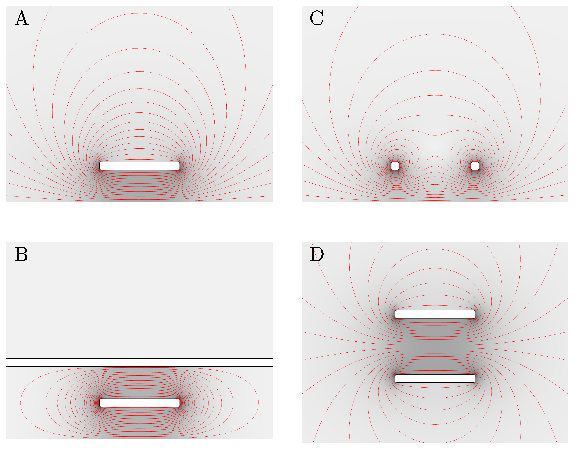
\includegraphics[width=0.8\textwidth]{cross-sections}
	\end{center}
	\caption{Cross section of some typical planar transmission line geometries,
  		including magnetic field lines of the TEM mode. A: microstrip, B: stripline, C: microslot, D: parallel plate transmission line}
	\label{fig:cross-sections}
\end{figure}

\subsection{Characteristic Impedance and Transport
Characteristics}\label{characteristic-impedance-and-transport-characteristics}

For TEM modes, it is possible to attribute a current and a voltage
amplitude to the travelling wave by integrating along the electric and
magnetic field lines in the cross section, respectively.
 While the absolute voltage and current amplitudes depend on the 
power transported by the wave, their
ratio (measured in $\Omega$) is a constant defined purely by the cross section
geometry and the dielectric and magnetic properties of the insulating
medium. This ratio is known as the characteristic impedance \m{Z_0} of
the wave guide. Coaxial cables are commonly designed for a
characteristic impedance of 50$\Omega$.

\subsection{Theory of TEM Wave Modes}\label{theory-of-tem-wave-modes}

Maxwell's curl equations couple the magnetic field \m{\mathbf{H}} and
the electric field \m{\mathbf{E}}. If we assume a harmonic time
evolution of the fields with angular frequency \m{\omega}, they become
%
\begin{eqnarray}
\nabla \times \mathbf{H} &= j \omega \epsilon \mathbf{E} \\
\nabla \times \mathbf{E} &= - j\omega \mu \mathbf{H}
\end{eqnarray}
%
where \m{j=\sqrt{-1}} is the imaginary unit, and \m{\epsilon} and
\m{\mu} represent the electric permittivity and magnetic permeability of
the insulating medium, respectively. In order to analyse a TEM mode, we
assume the axis of the transmission line to be aligned with the z
direction. The two curl equations can be combined to the Helmholtz
equation
%
\begin{equation}
(\nabla^2+k^2) \mathbf{E}  =0,
\end{equation}
%
where \m{k=\omega\sqrt{\mu\epsilon}} is the wave number. If we assume the
transverse components of the electric field to depend harmonically on $z$,
proportionally \m{e^{-j k z}}, it is easily shown that they
satisfy Laplace's equation, i.e.,
%
\begin{equation}
\left(\frac{\partial^2}{\partial x^2}+ \frac{\partial^2}{\partial y^2}\right) E_{x,y} = 0.
\end{equation}
A similar argument leads to the same result for the transverse magnetic
field. The electric and magnetic field distribution in the cross section
of a transmission line are therefore both solutions to Laplace's equation,
but they obey different boundary conditions.
For the electric field, we have\m{\mathbf{E} \cdot \mathbf{n}=0} at the
conductor surface,
and the magnetic field satisfies \m{\mathbf{H}\times \mathbf{n}=0},
where \m{\mathbf{n}} is the surface normal. It is useful to note that
the field distributions follow the same laws as  static fields. In particular,
this means that the field distribution for a TEM mode is
\textit{independent of the frequency}. TEM transmission lines are therefore
inherently broad-band devices, with no lower limit to the frequencies
they can carry. In theory, there is no upper limit for the propagation
of the TEM mode either; however, the excitation of TE and TM modes
complicates the situation at very high frequencies. For this reason,
coaxial transmission lines are only used up to frequencies of several
GHz. 

\subsection{Modelling of TEM modes}\label{modelling-of-tem-modes}

Since the transverse electric and magnetic field distributions for TEM
modes are solutions of the two-dimensional Laplace equation, they are
easily computed for any geometry using a finite element or finite
difference approach. Since the electric field is
curl-free, it can be represented as the gradient of an
electrostatic potential \m{\phi(x,y)}, which  satisfies the (scalar) Laplace
equation. Computing the transverse field distribution therefore reduces
to a simple Dirichlet problem, where fixed potential values must be
attributed to the conductor surfaces:
%
\begin{equation}
\nabla^2 \phi(x,y)=0 \quad\text{on }B, \qquad \phi=V_{1,2,\dots}\quad\text{on } \partial B_{1,2,\dots}, 
\end{equation}
where $B$ denotes the dielectric cross section, and $\partial B_{1,2,\dots}$
represent the conductor surfaces, and $V_{1,2,\dots}$ are the electrical
surface potentials.
The electric field of a propagating TEM mode is then given by
\begin{equation}
	\mathbf{E}=e^{-\gamma z} \left(-\frac{\partial\phi}{\partial x}, -\frac{\partial\phi}{\partial x},0\right),
\end{equation}
where $\gamma=\alpha+j k$ is the propagation constant, which describes both
the oscillatory propagation of the wave in the z direction with wave
number \m{k} and its gradual attenuation with decay constant \m{\alpha}.
\footnote{It should be noted that the foregoing treatment is only strictly exact in the 
limit $\alpha \ll k$. However, for transmission lines composed of polymer
dielectrics and good conductors, this is almost always true to a 
good approximation.}

The magnetic field distribution
is easily found using the the curl equations:
\begin{equation}
		\mathbf{H}=e^{-\gamma z} \left(\frac{1}{\eta}-\frac{j\alpha}{\omega\mu} \right)\left(\frac{\partial\phi}{\partial x}, -\frac{\partial\phi}{\partial y},0\right),
\end{equation}
where the characteristic impedance of the medium $\eta$ is given by
\begin{equation}
	\eta=\sqrt{\frac{\mu}{\epsilon}}.
\end{equation}
Note that in the case of $\alpha=0$, the magnetic and the electric field are \textit{in phase},
whereas a positive attenuation constant $\alpha>0$ leads to the magnetic field phase lagging behind the electric field.
%
The time-averaged power transported by the TEM wave is given by real part the 
Poynting vector as
\begin{equation}
	\Re(\mathbf{S})=\frac{1}{2}\Re(\mathbf{E}\times\mathbf{H}^\ast) = p_t\,\hat{\mathbf{z}},
\end{equation}
where the cross-sectional density of power $p_t(x,y)$ is
\begin{equation}
	p_t(x,y)=\frac{e^{-2\alpha z}}{2\eta} \left[\left(\frac{\partial\phi}{\partial x}\right)^2+\left(\frac{\partial\phi}{\partial y}\right)^2\right].
\end{equation}
The relative power loss per unit length is therefore given by
\begin{equation}
	 \frac{1}{p_t}\frac{\partial p_t}{\partial z} = -2\alpha.
\end{equation}

At every cross section of
the transmission line, it is possible to compute the electrical
potential difference between the two conductors by a path integral 
between the condutcor surfaces
%
\begin{equation}
V(z) = \oint_1^2 \mathbf{E}(x,y,z)\cdot \mathrm{d}\mathbf{s},
\end{equation}
%
Similarly, the current flowing in the conductor can be obtained using
Ampere's law
%
\begin{equation}
I(z) = \oint \mathbf{H}(x,y,z)\cdot \mathrm{d}\mathbf{s},
\end{equation}
%
where the integration path in this case is a closed loop around the
conductor. 


It is easily shown that the voltage and current thus obtained
satisfy the equations
%
\begin{eqnarray}
\frac{\mathrm{d}^2 V}{\mathrm{d}z^2} = \gamma^2 V(z) \\
\frac{\mathrm{d}^2 I}{\mathrm{d}z^2} = \gamma^2 I(z).
\end{eqnarray}
%
These equations are useful to describe the behaviour of transmission
lines when integrated into electrical circuit networks. In general, they
can be solved by a superposition of two waves travelling in opposite
directions:
%
\begin{eqnarray}
V(z) = V_0^+ e^{-\gamma z} + V_0^- e^{\gamma z} \\ 
I(z) = I_0^+ e^{-\gamma z} + I_0^- e^{\gamma z}.
\end{eqnarray}

The ratio
%
\begin{equation}
Z_0 = \frac{V_0^+}{I_0^+} = \frac{V_0^-}{I_0^-}
\end{equation}
%
is known as the characteristic impedance of the transmission line. Its
value depends entirely on the geometry of the transmission line cross
section and on the the dielectric and magnetic properties of the
insulator.



\subsubsection{Losses in Transmission
Lines}\label{losses-in-transmission-lines}

There are two main contributions to the power losses in a transmission
line. On the one hand, there are dielectric losses due to the repeated
polarisation and depolarisation of the insulating medium. These are
proportional to the magnitude of the electric fields. The dielectric
properties of most insulator materials are only very weakly frequency
dependent; the dissipated power therefore tends to be proportional to
the frequency. The dielectric dissipation of a material can be expressed
by an imaginary component in its dielectric permittivity
\m{\epsilon=\epsilon' - i \epsilon''}. Often, the loss tangent, defined
as \m{\tan \delta = \epsilon''/\epsilon'} is used in order to characterise
the material. A second (and, in the present context, often
dominant) source of losses is the finite conductivity of the metallic surfaces.
A plane electromagnetic wave impinging on an imperfect
conductor penetrates into it only to a finite depth \m{\delta_s}, known as
the skin depth. This is because the tangential component of the magnetic
field at the boundary induces in the surface a current which cancels the
magnetic field deeper inside the metal. Since this current is sustained
against a finite ohmic resistance, it disspates power from the electromagnetic wave. 
If the lateral dimensions of the transmission line are much larger
than the skin depth, it is possible to express the average dissipated power per
unit surface area as
%
\begin{equation}
P_\delta = \frac{1}{2}|H_\parallel|^2 R_s,
\end{equation}
%
where \m{R_s} is the surface resistance of the metal. It depends on the
conductivity $\sigma$ and the skin depth $\delta_s$ as
%
\begin{equation}
R_s = \frac{1}{\sigma \delta_s} = \sqrt{\frac{\omega\mu}{2\sigma}}.
\end{equation}
%
For pure Cu, \m{\sigma=5.9\cdot 10^7}S/m, which translates
into a surface resistance of about 10 m\m{\Omega} at 100 MHz, and about
35 m\m{\Omega} at 1 GHz. The losses lead to a gradual attenuation of a
travelling TEM mode, as reflected in the real part of the propagation
constant \m{\gamma}.


\subsection{Magnetic Fields in Planar TEM Transmission Lines}

The magnetic and electric field distributions of the TEM mode in some
planar transmission line geometries are shown in \fig{fig:cross-sections}. 
The stripline (\fig{fig:cross-sections}A) consists of a single conductor
 symmetrically bounded between two ground planes. The
magnetic field lines encircle the central conductor, producing two areas
of very high field homogeneity which can be used as sample locations for
NMR spectroscopy. The microstrip, shown in \fig{fig:cross-sections}B,
 exhibits a similar field geometry. However, since there is only 
 a single ground plane, the magnetic and electric fields penetrate into 
 the free space above. This
is less pronounced in practice than in the idealised computation shown
here, since the dielectric constant of the insulator means that the
electric field remains partially captured inside it. Nonetheless, the
open geometry can lead to radiation losses, which must be kept to a
minimum by external shielding. The difference in dielectric properties between
the insulator and the surrounding air also means that the propagating
mode in a microstrip is not strictly a TEM mode, and maintains some TE character.
This means that the relationship between the frequency and wavelength 
is not exactly linear, leading to frequency dispersion.

\fig{fig:cross-sections}C shows a microslot line. In this
case, there are two independent conductors, which can in principle carry
different electrical potentials. This geometry is therefore capable of
supporting more than one TEM mode. However, in the present context, only
the common mode shown in \fig{fig:cross-sections}C is of interest. Compared to the
similar microstrip geometry, the magnetic field is concentrated in the
space immediate above the pair of conductors.

Finally, \fig{fig:cross-sections}D shows a parallel plate transmission line (PTL). 
In this case, the two conductors are symmetrically placed above and below the centre line. 
The field lines extend into space on both sides of the structure, and are
compressed into a region of high field homogeneity in between the two 
conductors. 


\subsection{Transmission Line Detectors and Resonators}\label{transmission-line-resonators}
According to the correspondence principle, the sensitivity of an NMR detector
is directly related to the magnetic field it generates at the location of
the sample per unit current \cite{Hoult:1976dw}. In a transmission line
detector, sensitivity is therefore maximised if the lateral dimensions are chosen
as small as possible, and if the region of the largest magnetic field in the TEM
mode is filled with the sample. On the other hand, transmission lines with small 
cross sections tend to be more lossy. Many detector geometries therefore constrict the
width of the transmission line at the site of the sample.

In order to optimise the coupling of the detector to the spectrometer transmitter and 
receiver circuits, it is necessary to match its impedance to the standard impedance,
ususally 50$\Omega$. This is most commonly achieved by tuning the detector to a resonance
frequency very slightly above the desired Larmor frequency, and then nulling the resulting
positive reactance with a series capacitor. 

A transmission line stub of length $l$ with open ends (infinte termination impedance) will support
a manifold of eigenmodes, with frequencies that correspond to standing waves with current nodes
at the ends, i.e., an integer number of half waves must fit into $l$. The standing waves at these
frequencies exhibit voltage nodes at the locations of the current anti-nodes. This is convenient in 
NMR spectroscopy, because the most sensitive location of the resonator (at the 
magnetic field maxima) are automatically the ones where the electric field amplitude vanishes.
Well-designed resonant transmission line probes therefore exhibit only minimal sample heating, and 
are largely immune to quality factor degradation through dielectric losses.

Resonators can also be realised with other terminations. Often, one end of the transmission line
is short-circuited, rather than left open. This leads to a current anti-node at the shorted
end. 
In some cases, it is desirable to achive as uniform as possible a current distribution throughout
the length of the transmission line detector. This can be achieved by terminating both sides with
a capacitor. The desired eigenmode is then characterised by one capacitor being discharged
while the other is charged, and vice versa. The current amplitude in the transmission line
is then almost constant over its length. Obviously, only frequencies below the fundamental
mode of the corresponding open-ended transmission line resonator can be accessed in this manner.


